
% No need to change the first 4 lines of this file
\documentclass{uicthesi}

% This is the user manual for UICTHESI CLS, originally found
% at https://www.math.uic.edu/graduate/current/uicthesi, and
% modified by Pete Snyder <snyder@gmail.com> to match the
% current department requirements.
\usepackage{booktabs}
\usepackage{listings}
\usepackage{newlfont}
\usepackage{amsfonts}
\usepackage{amssymb}
\usepackage{euler}
\usepackage[xindy={glsnumbers=false},nonumberlist,acronym,nopostdot,nogroupskip,nomain]{glossaries}
\usepackage{xspace}
\usepackage[htt]{hyphenat}
\usepackage{float}
\usepackage{flushend}
\usepackage{footnote}
\usepackage{enumitem}
\usepackage{url}
\usepackage{caption}
\usepackage{graphicx}

\newglossarystyle{clong}{%
 \renewenvironment{theglossary}%
     {\begin{longtable}{p{.2\linewidth}p{.8\linewidth}}}%
     {\end{longtable}}%
  \renewcommand*{\glossaryheader}{}%
  \renewcommand*{\glsgroupheading}[1]{}%
  \renewcommand*{\glossaryentryfield}[5]{%
    \glstarget{##1}{##2} & ##3\glspostdescription\space ##5\\}%
  \renewcommand*{\glossarysubentryfield}[6]{%
     & \glstarget{##2}{\strut}##4\glspostdescription\space ##6\\}%
  %\renewcommand*{\glsgroupskip}{ & \\}%
}

\makesavenoteenv{tabular}
\makesavenoteenv{table}

% See https://www.ctan.org/pkg/glossaries for questions on this package.
% Refer to the acronyms you define here as \gls{nyc}.
%
% This make sure that this text:
%    The Ramones are from \gls{nyc}, thats right, \gls{nyc}.
% Gets output like this:
%    The Ramones are from New York City (NYC), thats right, NYC.
% And that a line in the acronyms section of your thesis has an entry like:
%    NYC         New York City
\newacronym{cms}{CMS}{Compact Muon Solenoid}
\newacronym{lhc}{LHC}{Large Hadron Collider}


\def\new@fontshape#1#2#3#4#5{\expandafter
     \edef\csname#1/#2/#3\endcsname{\expandafter\noexpand
                                 \csname #4\endcsname}}
\new@fontshape{cmr}{bx}{sc}{
      <5>cmcsc8 at 5pt%
      <6>cmcsc8 at 6pt%
      <7>cmcsc8 at 7pt%
      <8>cmcsc8%
      <9>cmcsc9%
      <10>cmcsc10%
      <11>cmcsc10 at 10.95pt%
      <12>cmcsc10 at 12pt%
      <14>cmcsc10 at 14.4pt%
      <17>cmcsc10 at 17.28%
      <20>cmcsc10 at 20.736pt%
      <25>cmcsc10 at 24.8832pt%
      }{}
\mathversion{normal}
\newcommand{\ams}{{$\cal{A}\cal{M}\cal{S}$}}
\newcommand{\amslatex}{{$\cal{A}\cal{M}\cal{S}$-\LaTeX{}}}
\newcommand{\amstex}{{$\cal{A}\cal{M}\cal{S}$-\TeX{}}}
\newcommand{\BibTeX}{{\rm B\kern-.05em{\sc i\kern-.025em b}\kern-.08em
    T\kern-.1667em\lower.7ex\hbox{E}\kern-.125emX}}
\newcommand{\uicthesi}{{$\mathbb{UICTHESI}$}}

\newcommand\bs{\char '134 }   % A backslash character for \tt font
\newcommand{\lb}{\char '173 } % A left brace character for \tt font
\newcommand{\rb}{\char '175 } % A right brace character for \tt font

% one or two other commands
\def\newfont#1#2{\@ifdefinable #1{\font #1=#2\relax}}
\def\symbol#1{\char #1\relax}

\makeglossaries

% Use this file to include custom commands...
\newcommand{\NumberOfRamonesMembers}{8\xspace}
\newcommand{\NumberOfRamonesAlbums}{14\xspace}

\newcommand{\RTR}{Rocket to Russia\xspace}
\newcommand{\EOFC}{End of the Century\xspace}




\begin{document}

% The title of the thesis
\title{Measuring Heavy Flavor Jet Production in PbPb and pp Collisions at $\sqrt{s_{NN}}$ = 5.02 TeV with the CMS Detector}

% Your full name
\author{Clayton Max Bennett}

% Mention all degrees you hold currently
\pdegrees{B.S. in Physics, University of Wisconsin Madison}
\pdegrees{M.S. in Physics, DePaul University}

% Probably no need to edit this
\degree{Doctor of Philosophy in Physics}

% Add your committee members, one per line, mentioning external universities
% where relevant
\committee{Olga Evdokimov, Chair and Advisor \\
Austin Baty \\
? \\
? \\
}

% No need to make any changes to the next 10 lines
\maketitle
\copyrightpage
\dedication

A brief dedication to someone you care about.  

\acknowledgment

A page or two so of shout-outs to people you appreciate.  Don't forget
your advisor and committee members!

I would like to thank everyone in my life for whom writing this dissertation was made possible.
Suppose the cross-section of life-changing interactions across many spacetime scales is given by
\begin{equation}
\label{eqn:clayton-cross-section}
d\sigma^{\text{Clayton}} = d\sigma^{\text{childhood}} \otimes d\sigma^{\text{college}} \otimes d\sigma^{\text{gradschool}}
\end{equation}  
The first term in \ref{eqn:clayton-cross-section} cannot exist without the love and support of my mother and father, Robin Schroeder and Randall Bennett, respectively, along with the loving support of my stepmother, Lisa Bennett.
This term also contains import contributions from my closest childhood friends, Sam Hemes and Connor Eccles.
Together, we made movies, we made music, and most importantly, we made memories.
The second term in \ref{eqn:clayton-cross-section} cannot be expressed accuratately without Emily Hegland -- the love of my life -- for whom I have been dedicated to since the day the we met.
This term also has non-negligable contributions from Tyson Williams, for whom inspired me first to study physics.
Finally, the last, and perhaps most important term in application to this thesis, derived from my time at UIC, immersing myself in the deep and beautiful laws of the universe:  I must first thank Olga Evdokimov, my advisor.
From you I learned so much, most of which is the 





\initials{CMB}

\authorcontributions

This section should give a rough overview of each chapter in the thesis,
highlighting your contributions.  Most importantly, for each one of your
papers you are quoting, this section should briefly describe what each author's
role / contribution was.

An example of ``Contribution of Authors'' section is on page 3 of the
University's guide to iThenticate\footnote{\url{http://grad.uic.edu/sites/default/files/pdfs/Introduction_to_Screening_Your_Thesis_or_Dissertation_using_iThenticate-final_a.pdf}}.
\setcounter{table}{0}	% fixes #3 (https://github.com/bitslab/uic-cs-thesis-template/issues/3#issuecomment-2455616743)
\tableofcontents
\listoftables
\listoffigures
%\printglossary[type=\acronymtype,title=LIST OF ABBREVIATIONS,style=clong]
\printglossaries[title=LIST OF ABBREVIATIONS]
\summary

One to two page summary of the entire work.  Like a long abstract.

% This is where you write the paper.  I've included a sample chapter
% below, to suggest a possible organization.  Just add references to the
% rest of your paper here.
\chapter{The Quark-Gluon Plasma}
\label{qgp}

\begin{frame}
  \frametitle{\textbf{Quantum Chromodynamics}}
  \begin{columns}
    \column{0.6\textwidth}
    \begin{itemize}
    \item \textbf{Quantum chromodynamics} (QCD) is a quantum field theory describing the \textbf{strong interaction} between \textbf{quarks} and \textbf{gluons}
    \item \textbf{Confinement}: fundamental feature of QCD
      \begin{align*}
        V_{\text{QCD}}(Q^2) = \color{gray}\underbrace{\color{black}-\cfrac{4}{3}\cfrac{\alpha_s(Q^2)}{r}}_{\text{QED-like short-range}} \color{black} + \color{gray} \underbrace{\color{black}\lambda r}_{\text{QCD long-range}}
      \end{align*}
    \item QCD is a quantum field theory with \textbf{asymptotic freedom}
    \end{itemize}
    \begin{align*}
      &\alpha_s(Q^2) = \cfrac{\alpha_s(\mu^2)}{1 + \left[\alpha_s(\mu^2)\frac{(11n_c - 2n_f)}{12\pi}\right]\ln\left(\frac{Q^2}{\mu^2}\right)} \\
      & \boxed{\lim_{Q \to \infty}\alpha_s(Q^2) \to 0}
    \end{align*}

    \begin{itemize}
    \item Large $Q^2 \to$ strong-force coupling gets \textbf{weaker}
    \end{itemize}



    \column{0.4\textwidth}
    \centering
    \begin{tikzpicture}
      \node{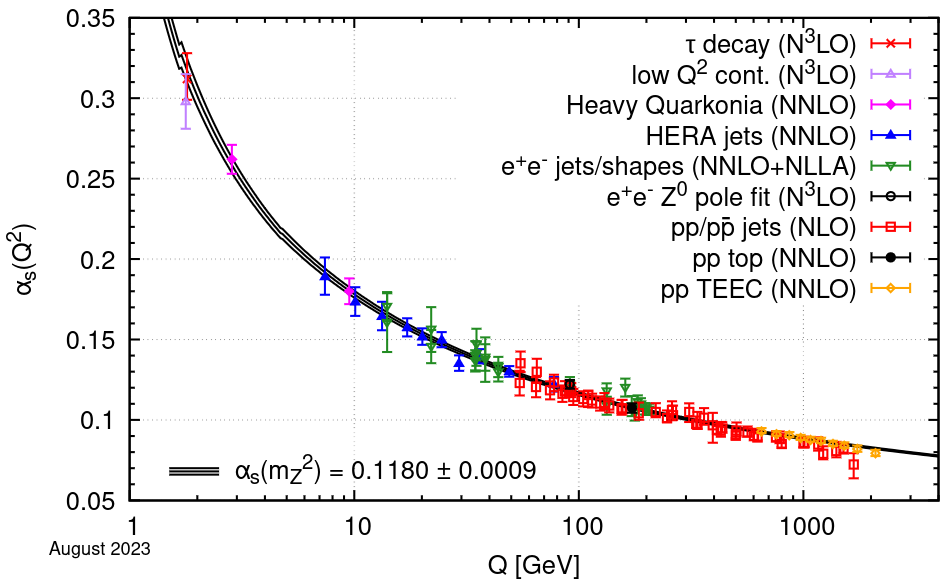
\includegraphics[width=0.9\textwidth]{running-coupling.png}};
      \node[font=\tiny,align=left] at (0.2,2.1) {\href{https://academic.oup.com/ptep/article/2022/8/083C01/6651666}{Prog. Theor. Exp. Phys. 2022, 083C01 (2022)}};
    \end{tikzpicture}

    \

    \

    \begin{columns}

      \column{0.33\textwidth}
      \resizebox{\textwidth}{\textwidth}{
        \begin{tikzpicture}
          \begin{feynman}
            \vertex (a) {\( q \)};
            \vertex[below right=of a] (b);
            \vertex[below left=of b] (c) {\( q \)};
            \vertex[right=of b] (d) {\( g \)};
            \diagram*{
              (a) -- [fermion] (b),
              (b) -- [fermion] (c),
              (b) -- [gluon] (d),
            };
          \end{feynman}
        \end{tikzpicture}
      }

      \column{0.33\textwidth}
      \resizebox{\textwidth}{\textwidth}{
        \begin{tikzpicture}
          \begin{feynman}
            \vertex (a) {\( g \)};
            \vertex[below right=of a] (b) ;
            \vertex[below left=of b] (c) {\( g \)};
            \vertex[right=of b] (d) {\( g \)};
            \diagram*{
              (a) -- [gluon] (b),
              (b) -- [gluon] (c),
              (b) -- [gluon] (d),
            };
          \end{feynman}
        \end{tikzpicture}
      }

      \column{0.33\textwidth}
      \resizebox{\textwidth}{\textwidth}{
        \begin{tikzpicture}
          \begin{feynman}
            \vertex (a) {\( g \)};
            \vertex[below right=of a] (b) ;
            \vertex[below left=of b] (c) {\( g \)};
            \vertex[above right=of b] (d) {\( g \)};
            \vertex[below right=of b] (e) {\( g \)};
            \diagram*{
              (a) -- [gluon] (b),
              (b) -- [gluon] (c),
              (b) -- [gluon] (d),
              (b) -- [gluon] (e),
            };
          \end{feynman}
        \end{tikzpicture}
      }

    \end{columns}
    

    
  \end{columns}
\end{frame}


\chapter{The Quark-Gluon Plasma}
\label{qgp}

\begin{frame}
  \frametitle{\textbf{Quantum Chromodynamics}}
  \begin{columns}
    \column{0.6\textwidth}
    \begin{itemize}
    \item \textbf{Quantum chromodynamics} (QCD) is a quantum field theory describing the \textbf{strong interaction} between \textbf{quarks} and \textbf{gluons}
    \item \textbf{Confinement}: fundamental feature of QCD
      \begin{align*}
        V_{\text{QCD}}(Q^2) = \color{gray}\underbrace{\color{black}-\cfrac{4}{3}\cfrac{\alpha_s(Q^2)}{r}}_{\text{QED-like short-range}} \color{black} + \color{gray} \underbrace{\color{black}\lambda r}_{\text{QCD long-range}}
      \end{align*}
    \item QCD is a quantum field theory with \textbf{asymptotic freedom}
    \end{itemize}
    \begin{align*}
      &\alpha_s(Q^2) = \cfrac{\alpha_s(\mu^2)}{1 + \left[\alpha_s(\mu^2)\frac{(11n_c - 2n_f)}{12\pi}\right]\ln\left(\frac{Q^2}{\mu^2}\right)} \\
      & \boxed{\lim_{Q \to \infty}\alpha_s(Q^2) \to 0}
    \end{align*}

    \begin{itemize}
    \item Large $Q^2 \to$ strong-force coupling gets \textbf{weaker}
    \end{itemize}



    \column{0.4\textwidth}
    \centering
    \begin{tikzpicture}
      \node{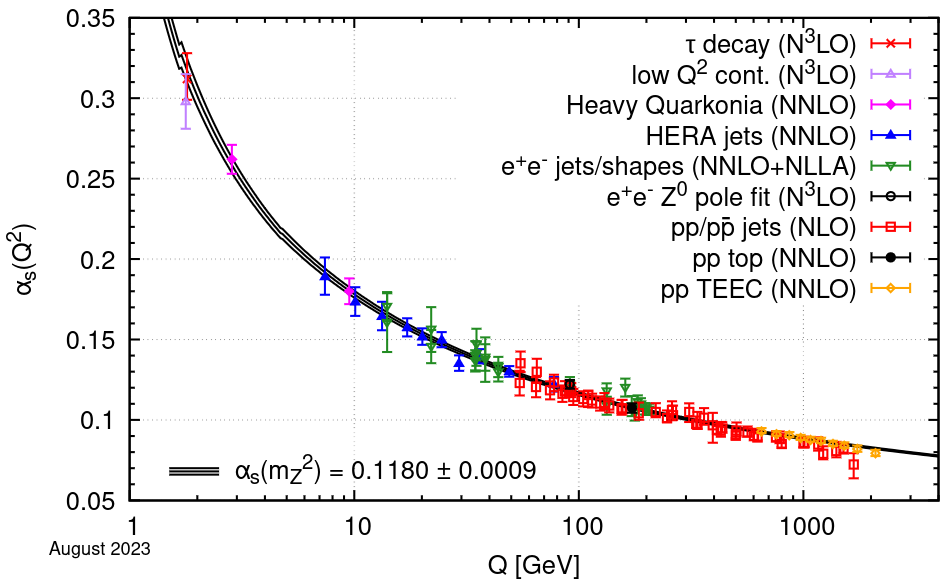
\includegraphics[width=0.9\textwidth]{running-coupling.png}};
      \node[font=\tiny,align=left] at (0.2,2.1) {\href{https://academic.oup.com/ptep/article/2022/8/083C01/6651666}{Prog. Theor. Exp. Phys. 2022, 083C01 (2022)}};
    \end{tikzpicture}

    \

    \

    \begin{columns}

      \column{0.33\textwidth}
      \resizebox{\textwidth}{\textwidth}{
        \begin{tikzpicture}
          \begin{feynman}
            \vertex (a) {\( q \)};
            \vertex[below right=of a] (b);
            \vertex[below left=of b] (c) {\( q \)};
            \vertex[right=of b] (d) {\( g \)};
            \diagram*{
              (a) -- [fermion] (b),
              (b) -- [fermion] (c),
              (b) -- [gluon] (d),
            };
          \end{feynman}
        \end{tikzpicture}
      }

      \column{0.33\textwidth}
      \resizebox{\textwidth}{\textwidth}{
        \begin{tikzpicture}
          \begin{feynman}
            \vertex (a) {\( g \)};
            \vertex[below right=of a] (b) ;
            \vertex[below left=of b] (c) {\( g \)};
            \vertex[right=of b] (d) {\( g \)};
            \diagram*{
              (a) -- [gluon] (b),
              (b) -- [gluon] (c),
              (b) -- [gluon] (d),
            };
          \end{feynman}
        \end{tikzpicture}
      }

      \column{0.33\textwidth}
      \resizebox{\textwidth}{\textwidth}{
        \begin{tikzpicture}
          \begin{feynman}
            \vertex (a) {\( g \)};
            \vertex[below right=of a] (b) ;
            \vertex[below left=of b] (c) {\( g \)};
            \vertex[above right=of b] (d) {\( g \)};
            \vertex[below right=of b] (e) {\( g \)};
            \diagram*{
              (a) -- [gluon] (b),
              (b) -- [gluon] (c),
              (b) -- [gluon] (d),
              (b) -- [gluon] (e),
            };
          \end{feynman}
        \end{tikzpicture}
      }

    \end{columns}
    

    
  \end{columns}
\end{frame}



% No need to make any changes to this file below this line.
\newpage
\bibformb
%\bibliographystyle{ieeetr}
\bibliography{thesis}
\newpage
\vita
\begin{singlespace}
    \begin{description}[labelwidth=4cm,leftmargin=4.2cm,itemsep=1em]

        % Your full name bere
        \item[NAME] Clayton Max Bennett

        % Put any degrees you have, in the form of: Degree type, Degree Field, Institution, City, State, Year
        \item[EDUCATION] B.S., Physics, University of Wisconsin Madison, Madison, WI, 2015
        \item[EDUCATION] M.S., Physics, DePaul University, Chicago, IL, 2020
          
        % If you have any teaching experience, put it here
        \item[TEACHING] Music lessons (CS342, Summer 1980)

        \item[PUBLICATIONS]
            \begin{itemize}[label={},listparindent=0pt,itemindent=0pt,leftmargin=0pt,itemsep=1em,parsep=0pt,topsep=0pt,partopsep=0pt]

                % Place each publication you've completed, no matter how trivial,
                % here.  Match the formatting below, to match the expected formatting.
                \item Author 1, Author 2, and Author 3. %
                ``Paper title 1.'' %
                In Proceedings of the CONFERENCE NAME (CONFERENCE ABBR, YEAR).

                \item Author 1, Author 2, and Author 3. %
                ``Paper title 2.'' %
                In Proceedings of the CONFERENCE NAME (CONFERENCE ABBR, YEAR).

                % etc...
            \end{itemize}
    \end{description}
\end{singlespace}

\end{document}
